\chapter{Datos y Representación de la Información}
\label{cap:datos}

El presente capítulo detalla el flujo de datos
implementado para el entrenamiento y evaluación del sistema de
transcripción, además del origen de los mismos. Se describe el conjunto
de datos utilizado, justificando su idoneidad para el problema polifónico
y, más específicamente, el caso concreto del piano. A continuación, se
especifica el preprocesamiento de la señal de audio acústica para generar
la representación de entrada y, finalmente, se define el diseño del
vocabulario discreto que permite codificar los eventos musicales como
secuencias de \textit{tokens}.

% -----------------------------------------------------------
\section{Conjunto de Datos}
\label{sec:conjunto_datos}
% -----------------------------------------------------------

Para el entrenamiento, validación y evaluación del sistema desarrollado,
se ha empleado el conjunto de datos MAESTRO (\textit{MIDI and Audio
Edited for Synchronous TRacks and Performances})
\cite{hawthorne2018enabling}. La elección de este corpus se fundamenta
en su posición como el estándar actual en el estado del arte para tareas
de transcripción de piano polifónico, superando ampliamente predecesores
como MAPS en términos tanto de volumen como de calidad acústica y
precisión de alineamiento.

\subsection{Descripción del corpus}

El conjunto de datos MAESTRO consta aproximadamente de 200 horas de
interpretaciones virtuosas de obras de piano clásico. La característica
más crítica de este corpus para el modelado secuencia a secuencia es la
naturaleza de su captura: las interpretaciones fueron registradas
utilizando pianos acústicos equipados con el sistema Yamaha Disklavier.
Este mecanismo permite capturar simultáneamente la señal de audio
acústica de alta fidelidad y los eventos físicos de las teclas y pedales
con una precisión temporal inferior a los 3 milisegundos, tal y como se
ilustra en la Figura~\ref{fig:audio_midi_maestro}.

\clearpage

\begin{figure}[htbp]
    \centering
    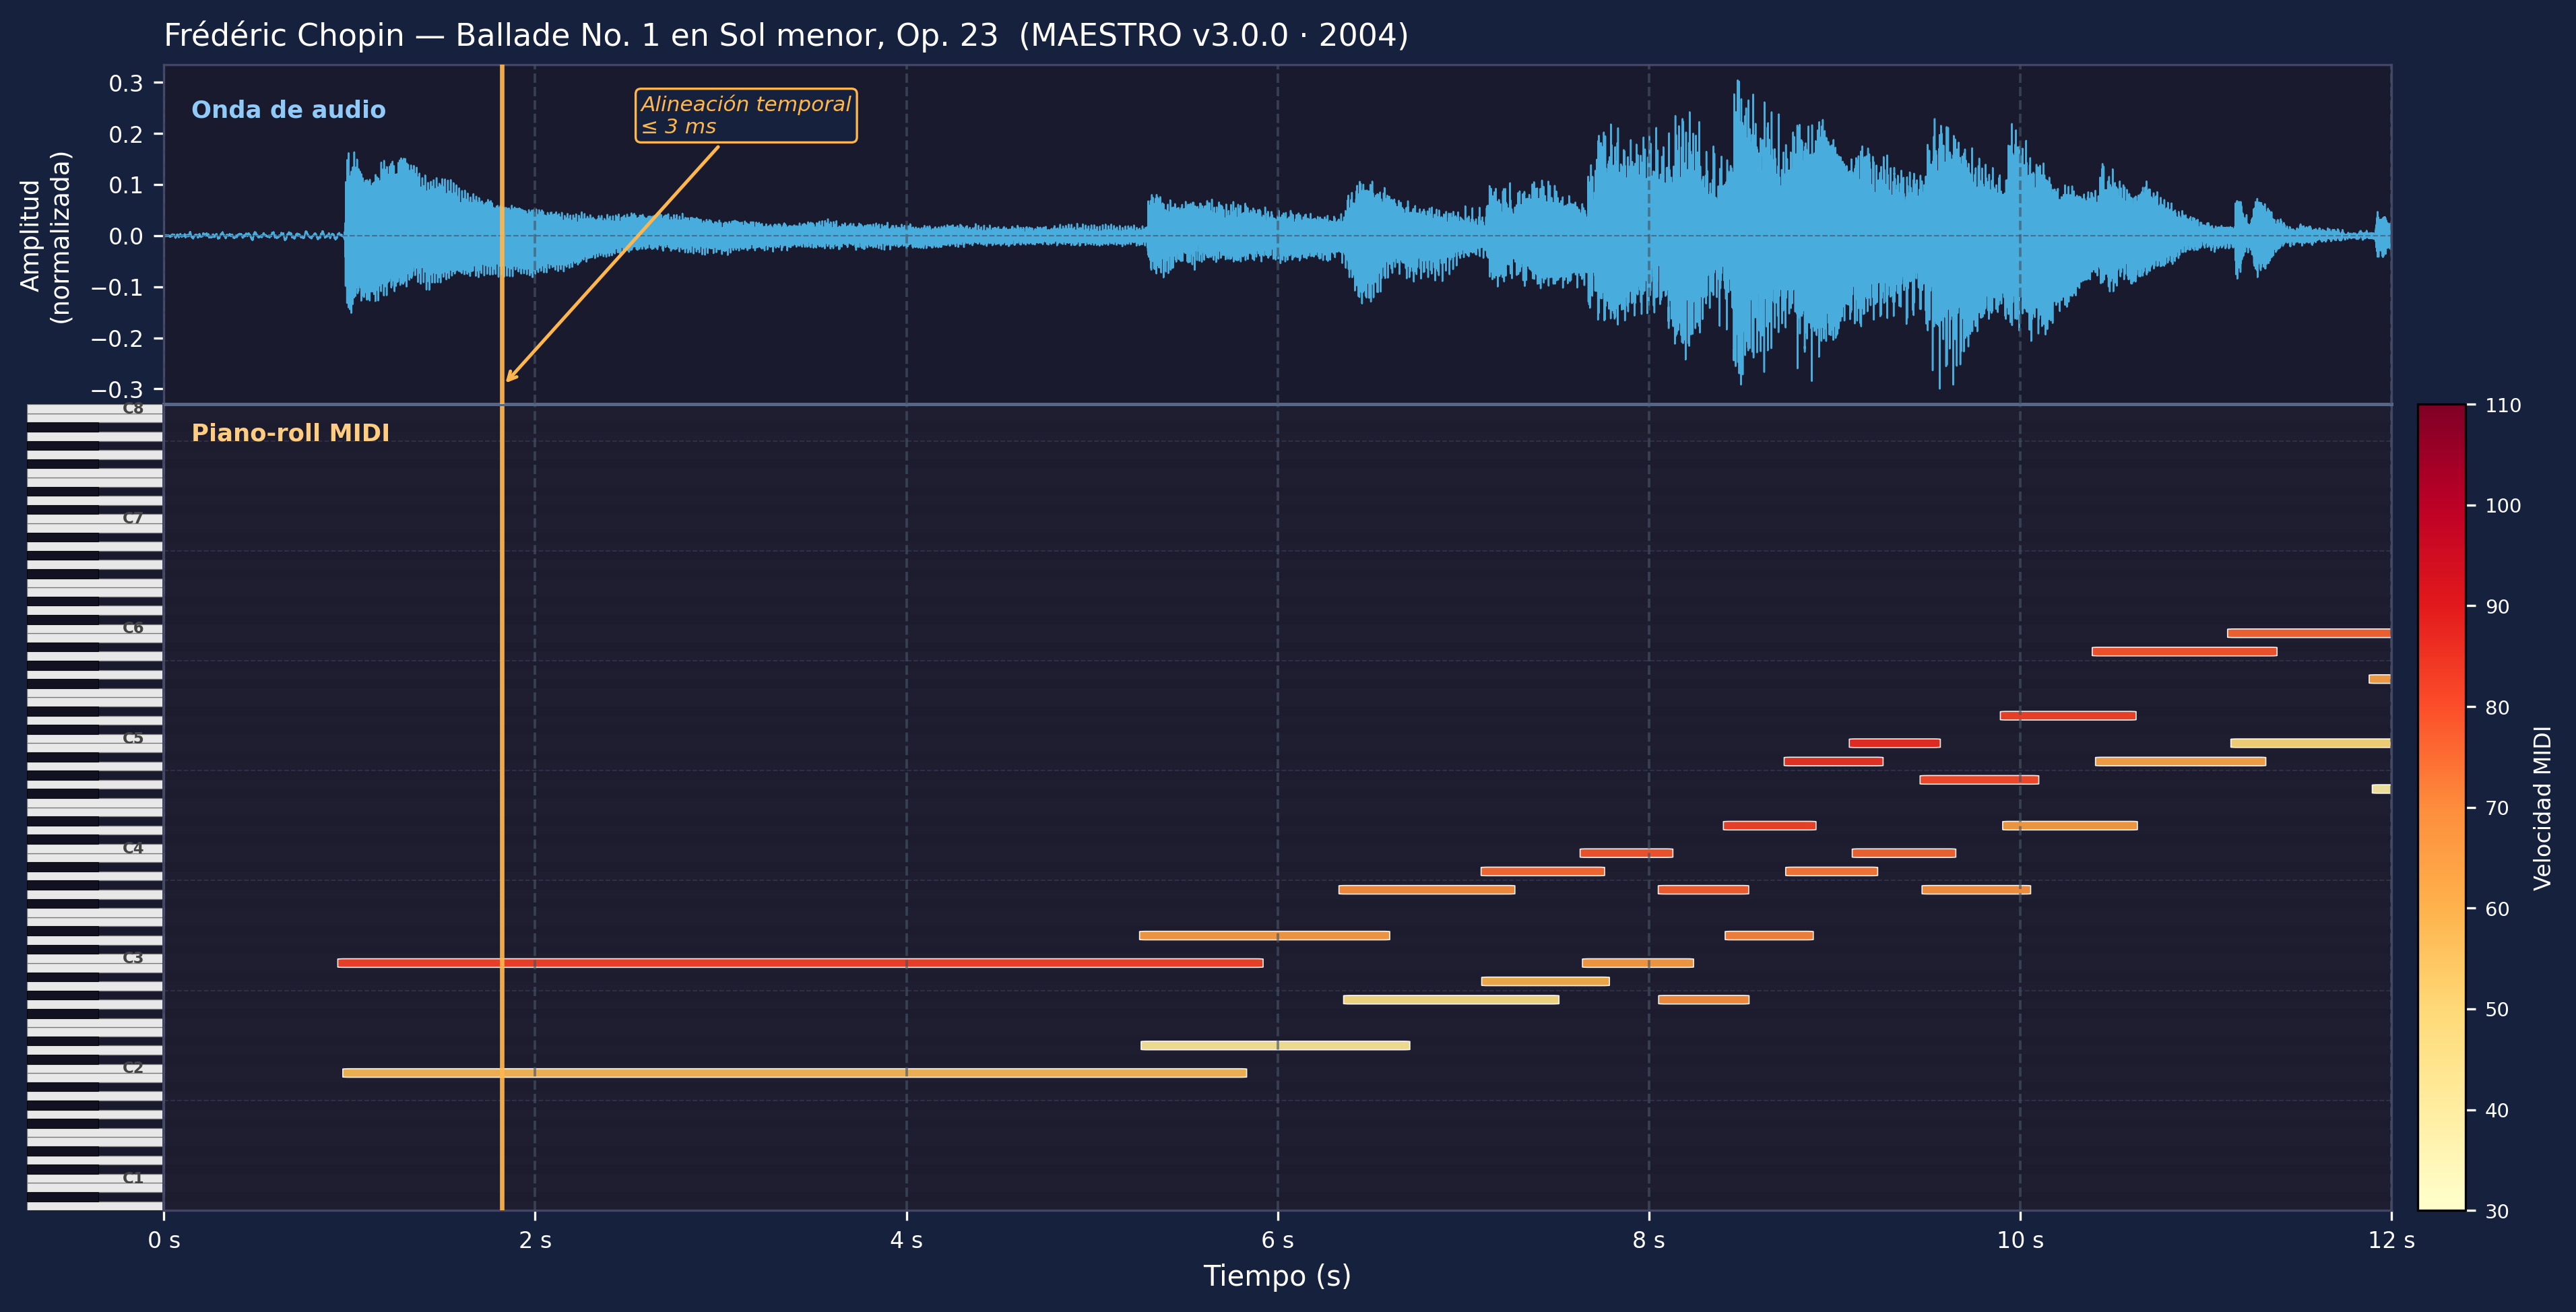
\includegraphics[width=\textwidth]{figs/audio_midi_alignment.png}
    \caption{Alineación temporal entre la señal de audio y el
    \textit{piano-roll} MIDI en una interpretación del corpus MAESTRO
    (Frédéric Chopin, \textit{Ballade} n.º~1 en Sol menor, Op.~23).
    Panel superior: forma de onda normalizada de la grabación acústica.
    Panel inferior: \textit{piano-roll} MIDI correspondiente, con las
    notas coloreadas según su velocidad de pulsación. La línea vertical
    naranja señala un ataque concreto, evidenciando la precisión de
    alineación inferior a 3~ms que caracteriza al \textit{dataset}
    MAESTRO.}
    \label{fig:audio_midi_maestro}
\end{figure}

Esta alineación temporal precisa entre el dominio continuo (el audio WAV)
y el dominio simbólico (los eventos MIDI que lo representan) proporciona
la verdad de referencia (\textit{ground truth}) indispensable para supervisar
el entrenamiento de la red neuronal. El corpus incluye una enorme
variabilidad de condiciones acústicas reales, como el solapamiento de
frecuencias, resonancias armónicas complejas producidas por el uso
intensivo del pedal de \textit{sustain} y un amplio rango dinámico en la
intensidad de pulsación de las teclas (\textit{velocity}), oscilando
desde el \textit{pianissimo} hasta el \textit{fortissimo}. Esta riqueza
acústica es vital para que el modelo aprenda a desentramar la polifonía
densa en lugar de memorizar patrones sintéticos.

\subsection{Partición de los datos}

Para garantizar una metodología de experimentación rigurosa y la
capacidad de generalización del modelo, el conjunto de datos se ha
dividido en tres subconjuntos mutuamente excluyentes: entrenamiento
(\textit{train}), validación (\textit{validation}) y prueba
(\textit{test}). Se ha respetado la partición oficial recomendada por
los creadores del \textit{dataset}, la cual distribuye los datos en
proporciones aproximadas de 80\,\%, 10\,\% y 10\,\%, respectivamente.

Es fundamental destacar que esta partición no se realiza a nivel de
fragmento de audio, sino a nivel de composición musical. Esto significa
que ninguna obra musical que aparezca en el conjunto de entrenamiento
estará presente en los conjuntos de validación o prueba. Esta restricción
de separación estricta (\textit{zero data leakage}) es una decisión de
ingeniería crítica que evita que el modelo memorice la estructura de una
pieza específica o las particularidades de una grabación concreta. De
este modo, las métricas obtenidas durante la evaluación reflejan
auténticamente la capacidad del sistema para transcribir piezas musicales
nunca antes vistas. Las estadísticas detalladas de cada subconjunto se
recogen en la Tabla~\ref{tab:maestro_splits} y serán referenciadas en el
Capítulo~\ref{cap:resultados} durante el análisis experimental.

\begin{table}[htbp]
    \centering
    \renewcommand{\arraystretch}{1.2}
    \begin{tabular}{l|r|r|r|r|r}
        \textit{Split} &
        \textit{Performances} &
        \textit{Compositions}\textsuperscript{*} &
        \makecell{\textit{Duration},\\\textit{hours}} &
        \textit{Size}, GB &
        \makecell{\textit{Notes},\\\textit{millions}} \\
        \hline
        \textit{Train}      & 954  & 295 & 140.1 & 83.6  & 5.06 \\
        \textit{Validation} & 105  &  60 &  15.3 &  9.1  & 0.54 \\
        \textit{Test}       & 125  &  75 &  16.9 & 10.1  & 0.57 \\
        \textbf{Total} & \textbf{1184} & \textbf{430} &
        \textbf{172.3} & \textbf{102.8} & \textbf{6.18} \\
    \end{tabular}
    \caption{Estadísticas de las particiones (\textit{splits}) del
    conjunto de datos MAESTRO \cite{hawthorne2018enabling}.
    \textsuperscript{*}Una misma obra musical puede estar interpretada
por varios pianistas distintos dentro del corpus; el recuento de
composiciones únicas es por tanto una estimación basada en los
metadatos oficiales del \textit{dataset}}
    \label{tab:maestro_splits}
\end{table}

% -----------------------------------------------------------
\section{Representación de entrada: Dominio Acústico}
\label{sec:dominio_acustico}
% -----------------------------------------------------------

Como se describe en la Sección~\ref{sec:representacion_audio}, la
entrada al modelo es un espectrograma Log-Mel obtenido a partir de la
señal de audio en crudo. Esta sección no abarca
la justificación conceptual de dicha representación, sino que especifica
los parámetros concretos adoptados en este sistema y el flujo de
preprocesamiento que los produce.

\subsection{Preprocesamiento de la señal}

El primer paso del flujo de datos consiste en la homogeneización de los
archivos de audio de entrada. Todas las grabaciones se convierten de
formato estereofónico a monofónico (mezcla de canales) para reducir la
carga computacional, dado que la información espacial estéreo no aporta
ventajas significativas para la extracción de características armónicas
\cite{muller2021fundamentals}. A continuación, las señales se remuestrean
a una frecuencia constante de $f_s = 16000\,\mathrm{Hz}$. Esta tasa de
muestreo es suficiente para capturar el contenido armónico relevante del
piano (cuyo rango tonal fundamental llega hasta aproximadamente
4186\,Hz), cumpliendo con el teorema de Nyquist-Shannon
\cite{shannon1949communication}.

Dado que el corpus MAESTRO contiene interpretaciones de hasta varios
minutos de duración, y con el objetivo de mantener la viabilidad
computacional del entrenamiento, se aplica una truncación de la
secuencia de audio a un máximo de 4\,096 tramas espectrales
(equivalente a aproximadamente 82 segundos). Las secuencias más
cortas se rellenan con ceros hasta alcanzar la longitud del elemento
más largo del lote (\textit{batch}). Los detalles de esta estrategia
y su variación entre experimentos se describen en el
Capítulo~\ref{cap:implementacion}.

\subsection{Parámetros del espectrograma Log-Mel}

Siguiendo la representación introducida en la
Sección~\ref{sec:representacion_audio}, el espectrograma Log-Mel se
calcula con los parámetros recogidos en la
Tabla~\ref{tab:parametros_espectrograma}. A continuación se justifica
cada elección en el contexto específico de la transcripción de piano.

El tamaño de ventana $N_{FFT} = 2048$ muestras (equivalente a 128\,ms)
proporciona una resolución frecuencial de
$f_s / N_{FFT} \approx 7{,}8\,\mathrm{Hz}$ por banda, suficiente para
distinguir notas próximas en el registro grave del instrumento, donde los
armónicos están más juntos. El \textit{hop size} de 320~muestras
(20\,ms por trama) establece la resolución temporal de la representación:
a esta granularidad, el modelo puede capturar transitorios de ataque con
suficiente precisión para la detección de \textit{onsets} dentro de la
ventana de tolerancia de $\pm 50\,\mathrm{ms}$ empleada en la evaluación
estándar (véase Sección~\ref{sec:metricas}). El banco de 229~filtros Mel,
delimitado entre $f_{min} = 31\,\mathrm{Hz}$ y
$f_{max} = 8000\,\mathrm{Hz}$, cubre íntegramente el rango tonal del
piano (desde A0 a 27{,}5\,Hz hasta C8 a 4186\,Hz) incluyendo los
armónicos perceptivamente más relevantes. Esta configuración de
parámetros sigue la práctica habitual en sistemas de AMT de alto
rendimiento evaluados sobre el corpus MAESTRO
\cite{kong2021high, purwins2019deep}.

Finalmente, los valores de energía del espectrograma se normalizan al
rango $[0, 1]$ mediante dos pasos sucesivos: primero se aplica una
conversión logarítmica a decibelios con referencia al máximo de la señal
y un rango dinámico de 60\,dB, obteniendo valores en el intervalo
$[-60, 0]\,\mathrm{dB}$; a continuación, dichos valores se reescalan
linealmente a $[0, 1]$. Esta normalización homogeneiza la distribución
de la entrada entre piezas de distinta intensidad media y estabiliza el
proceso de entrenamiento.

\begin{table}[htbp]
    \centering
    \renewcommand{\arraystretch}{1.3}
    \begin{tabular}{l l p{7.5cm}}
        \hline
        \textbf{Parámetro} & \textbf{Valor} & \textbf{Descripción} \\
        \hline
        Frecuencia de muestreo ($f_s$)      & 16\,000\,Hz   &
            Tasa de muestreo de la señal monofónica de entrada. \\
        Tamaño de ventana ($N_{FFT}$)        & 2048 muestras &
            Equivalente a 128\,ms de resolución temporal por trama. \\
        Tamaño de salto (\textit{hop size})  & 320 muestras  &
            Equivalente a 20\,ms de desplazamiento entre ventanas. \\
        Tipo de ventana                      & \textit{Hann} &
            Función aplicada para suavizar los extremos de la trama. \\
        Filtros Mel ($N_{mels}$)             & 229           &
            Cubre holgadamente las 88 teclas del piano y sus armónicos. \\
        Frecuencia mínima ($f_{min}$)        & 31\,Hz        &
            Límite inferior; próximo a la nota A0 del piano. \\
        Frecuencia máxima ($f_{max}$)        & 8000\,Hz      &
            Límite superior dictado por la frecuencia de Nyquist. \\
        \hline
    \end{tabular}
    \caption{Parámetros de configuración para el cálculo del espectrograma
    Log-Mel.}
    \label{tab:parametros_espectrograma}
\end{table}

% -----------------------------------------------------------
\section{Representación de salida: Dominio Simbólico}
\label{sec:dominio_simbolico}
% -----------------------------------------------------------

Para que el modelo Transformer pueda generar eventos musicales mediante
un enfoque de traducción de secuencia a secuencia, es necesario
transformar los archivos MIDI continuos en una secuencia unidimensional
de \textit{tokens} discretos. Para ello, se ha diseñado un vocabulario
personalizado inspirado en representaciones estándar de la literatura
\cite{oore2020time}.

\subsection{Diseño del vocabulario (\textit{Tokenization})}

El vocabulario desarrollado consta de un total de 311~\textit{tokens}
únicos. Esta dimensionalidad reducida resulta eficiente para la capa de
clasificación final de la red neuronal. Los \textit{tokens} se
estructuran en familias que cubren integralmente los atributos musicales
del piano:

\begin{itemize}
    \item \textbf{\textit{Tokens} de gestión de secuencia:} El
    \textit{token} \texttt{<pad>} (índice~0) homogeneiza la longitud de
    los tensores en los lotes de entrenamiento (\textit{batches}). Los
    \textit{tokens} \texttt{<sos>} (\textit{Start of Sequence},
    índice~309) y \texttt{<eos>} (\textit{End of Sequence}, índice~310)
    delimitan las fronteras de la generación autorregresiva.

    \item \textbf{Activación y desactivación de notas
    (\textit{Note-On\,/\,Note-Off}):} Se restringe el rango tonal a las
    88~teclas del piano estándar, desde A0 (índice MIDI~21) hasta C8
    (índice MIDI~108), lo que se traduce en 88~\textit{tokens} de
    \textit{Note-On} (índices 1--88) y 88~\textit{tokens} de
    \textit{Note-Off} (índices 89--176).

    \item \textbf{Desplazamiento temporal (\textit{Time-Shift}):} En
    lugar de predecir el estado del piano en cada instante físico, el
    modelo predice saltos en el tiempo con una resolución de
    $\Delta t = 1{,}0 \times 10^{-2}\,\mathrm{s}$. El vocabulario
    incluye 100~\textit{tokens} de \textit{Time-Shift} (índices
    177--276), permitiendo codificar esperas de hasta 1~segundo por
    \textit{token}.

    \item \textbf{Dinámica (\textit{Velocity}):} La intensidad de
    pulsación, codificada en MIDI en 128~valores (0--127), se cuantiza
    linealmente en 32~niveles o \textit{bins} (índices 277--308). Esta
    reducción mitiga la dispersión de los datos dinámicos sin una pérdida
    perceptible de expresividad musical.
\end{itemize}

\subsection{Gramática de eventos y lógica de decodificación}

La transformación de notas MIDI a \textit{tokens} requiere una ordenación
cronológica estricta para garantizar la viabilidad del entrenamiento
autorregresivo. Los eventos se ordenan por su marca de tiempo y, ante
empates temporales, se otorga prioridad absoluta a los eventos
\textit{Note-Off} sobre los \textit{Note-On}. Esta regla gramatical
previene colisiones lógicas y asegura que una tecla finalice su
vibración antes de volver a ser percutida en el mismo instante.

El proceso inverso (decodificación de \textit{tokens} a archivo MIDI)
implementa una máquina de estados para rastrear las notas activas. Esta
lógica incluye mecanismos de seguridad robustos: el cierre forzado de una
nota si se predice un nuevo \textit{Note-On} sin \textit{Note-Off} previo,
y un proceso de limpieza final que apaga todas las notas activas al
predecir el \textit{token} \texttt{<eos>}, evitando corrupciones en el
archivo MIDI resultante.